
\begin{figure}[h]
    \centering
    \begin{tabular}{cc}
    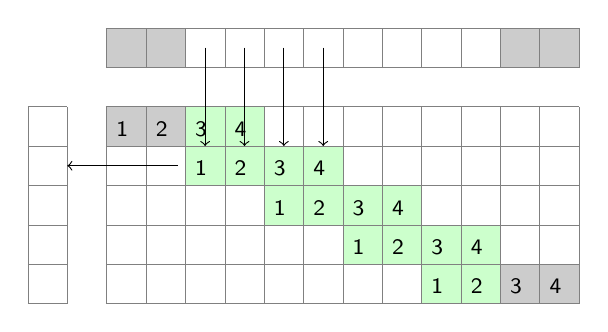
\begin{tikzpicture}[font=\footnotesize\sffamily]
        \fill[black!20!white] (1,3) rectangle (2,3.5);
        \fill[black!20!white] (6,3) rectangle (7,3.5);

        \foreach \x/\y in {1/2, 2/1.5, 3/1, 4/0.5, 5/0}
            \fill[green!20!white] (\x, \y) rectangle (\x + 2, \y + 0.5);

        \fill[black!20!white] (1,2) rectangle (2,2.5);
        \fill[black!20!white] (6,0) rectangle (7,0.5);

        \foreach \x/\y in {1/2, 2/1.5, 3/1, 4/0.5, 5/0}
        {
            \node[above right] at (\x + 0.0, \y) {1};
            \node[above right] at (\x + 0.5, \y) {2};
            \node[above right] at (\x + 1.0, \y) {3};
            \node[above right] at (\x + 1.5, \y) {4};
        }

        \draw[step=0.5cm,gray,very thin] (0,0) grid (0.5,2.5);
        \draw[step=0.5cm,gray,very thin] (0.99,2.99) grid (7,3.5);
        \draw[step=0.5cm,gray,very thin] (0.99,0) grid (7,2.5);
        \draw [->] (2.25,3.25) -- (2.25,2);
        \draw [->] (2.75,3.25) -- (2.75,2);
        \draw [->] (3.25,3.25) -- (3.25,2);
        \draw [->] (3.75,3.25) -- (3.75,2);
        \draw [->] (1.9,1.75) -- (0.5,1.75);
    \end{tikzpicture} &
    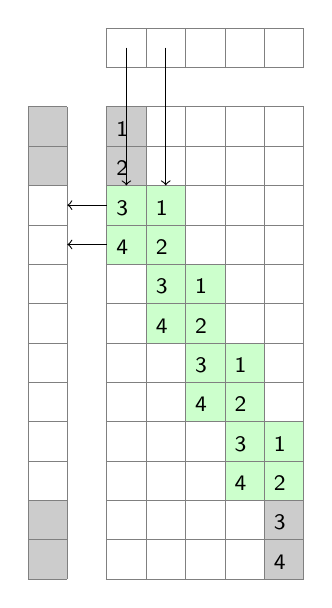
\begin{tikzpicture}[font=\footnotesize\sffamily]
        \fill[black!20!white] (0,5) rectangle (0.5,6);
        \fill[black!20!white] (0,0) rectangle (0.5,1);

        \foreach \y/\x in {4/1, 3/1.5, 2/2, 1/2.5, 0/3}
            \fill[green!20!white] (\x, \y) rectangle (\x + 0.5, \y + 2);

        \fill[black!20!white] (1,5) rectangle (1.5,6);
        \fill[black!20!white] (3,0) rectangle (3.5,1);

        \foreach \y/\x in {4/1, 3/1.5, 2/2, 1/2.5, 0/3}
        {
            \node[above right] at (\x, \y + 1.5) {1};
            \node[above right] at (\x, \y + 1.0) {2};
            \node[above right] at (\x, \y + 0.5) {3};
            \node[above right] at (\x, \y) {4};
        }

        \draw[step=0.5cm,gray,very thin] (0.99,6.49) grid (3.5,7);
        \draw[step=0.5cm,gray,very thin] (0,0) grid (0.5,6);
        \draw[step=0.5cm,gray,very thin] (0.99,0) grid (3.5,6);
        \draw [->] (1.25,6.75) -- (1.25,5);
        \draw [->] (1.75,6.75) -- (1.75,5);
        \draw [->] (1,4.75) -- (0.5,4.75);
        \draw [->] (1,4.25) -- (0.5,4.25);
    \end{tikzpicture} \\[6pt]
    (a) Convolution & (b) Deconvolution
    \end{tabular}
    \caption{Convolution with stride 2 in 1D \citep{shi_is_2016}}
    \label{fig:1d_strided_conv}
\end{figure}
